\chapter{Reaction Kinetics}
\section{Homework: Reaction Kinetics}
\subsection{Redox}
\subsubsection{Problem}
Hydrogen peroxide reacts with acidified iodide ions, liberating iodine.
In investigations of this reaction, the following results were
obtained (Table~\ref{tab:h2o2}).
\begin{table}[htpb]
	\centering
	\footnotesize
	\begin{tabular}{l r r r r}
		\toprule
		Experiment & \ch{[H2O2]}/\unit{\milli\conc} & \ch{[I^-]}/\unit{\milli\conc} & \ch{[H^{+}]}/\unit{\milli\conc} & Initial rate/\unit{\milli\concrate} \\
		\midrule
		1          & \num{10.0}                     & \num{9.0}                     & \num{10.0}                      & \num{2.30e-3}                       \\
		2          & \num{34.0}                     & \num{9.0}                     & \num{10.0}                      & \num{7.82e-3}                       \\
		3          & \num{34.0}                     & \num{13.5}                    & \num{10.0}                      & \num{1.75e-2}                       \\
		4          & \num{34.0}                     & \num{9.0}                     & \num{24.0}                      & \num{7.82e-3}                       \\
		\bottomrule
	\end{tabular}
	\caption{Results for reaction between \ch{H2O2} and \ch{I-}}
	\label{tab:h2o2}
\end{table}

\begin{enumerate}
	\item Determine the rate equation of this reaction.
	\item Calculate the rate constant and state its units.
\end{enumerate}

\subsubsection{Solution}
Since the initial rate increases linearly with \ch{[H2O2]}, the reaction
is first-order w.r.t. \ch{[H2O2]}. The reaction is second-order w.r.t. \ch{[I^-]}
and zeroth-order w.r.t. \ch{[H^{+}]}. Therefore, the rate equation is (Equation~\ref{eq:rateeq-h2o2})

\begin{equation}
	\color{accent}
	v = k \ch{[H2O2]} {\ch{[I^-]}}^2
	\label{eq:rateeq-h2o2}
\end{equation}

We can substitute the values from Experiment 1 into Equation~\ref{eq:rateeq-h2o2}.
\begin{align*}
	\num{2.30e-3} & = k \left(10.0\right) \ab(9.0)^2                         \\
	k             & = \f{\num{2.30e-3}}{\num{810.0}}                         \\
	              & = \color{accent} \qty{2.84e-6}{mmol^{-2}.dm^{-6}.s^{-1}} \\
\end{align*}

\subsection{Decomposition Graphs}
\subsubsection{Problem}
The decomposition of \ch{N2O4} is found to be \textbf{first-order}
with respect to \ch{[N2O4]} (Figure~\ref{fig:graphs}).
Which of the following graphs confirms the above finding? For the graphs that are incorrect, copy the axes
and sketch the correct shape of the graph.
\begin{figure}
	\centering
	\includegraphics[width=0.90\linewidth]{assets/06_n2o4.png}
	\caption{Various graphs of the decomposition of \ch{N2O4}}
	\label{fig:graphs}
\end{figure}

\begin{itemize}
	\item Graph \textbf{A} is {\color{accent} incorrect}. It illustrates a zeroth-order decomposition instead of a first-order one. The correct shape is:
	      \begin{center}
		      \begin{tikzpicture}
			      \begin{axis}[
					      ticks=none,
					      xmin=0,ymin=0,xmax=3,ymax=3,
					      xlabel={\(\slf{\ch{[N2O4]}}{\unit{\conc}}\)},
					      ylabel={\(\slf{v}{\unit{\concrate}}\)},
				      ]
				      \addplot+[dotted]{1.5};
				      \addplot{x};
			      \end{axis}
		      \end{tikzpicture}
	      \end{center}
	\item Graph \textbf{B} is {\color{accent} correct}. Since \(v = -\odv{\ch{[N2O4]}}/{t}\)
	      and \ch{N2O4} undergoes first-order decomposition, \ch{[N2O4]} should decrease
	      linearly too.
	\item Graph \textbf{C} is {\color{accent} correct}. Since \(v = k\ch{[N2O4]}\),
	      \(k = \slf{v}{\ch{[N2O4]}}\), a constant.
	\item Graph \textbf{D} is {\color{accent} incorrect}. The graph of \(v\) against
	      \ch{[N2O4]} is linear, so the graph of \(\log v\) against \(\log \ch{[N2O4]}\)
	      should follow a logarithmic curve:
	      \begin{center}
		      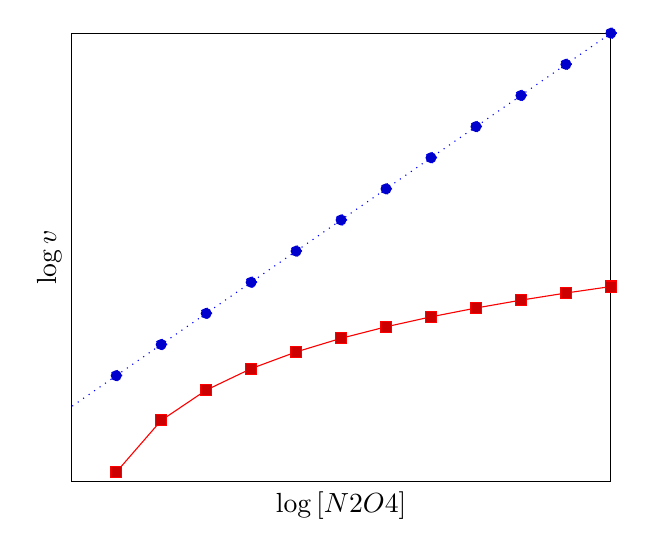
\begin{tikzpicture}
			      \begin{axis}[
					      ticks=none,
					      xmin=0,ymin=-1,xmax=5,ymax=5,
					      xlabel={\(\log \ch{[N2O4]}\)},
					      ylabel={\(\log v\)},
					      ticks=none,
				      ]
				      \addplot+[dotted]{x};
				      \addplot{ln x};
			      \end{axis}
		      \end{tikzpicture}
	      \end{center}
\end{itemize}

\subsection{Carbon Dating}
\subsubsection{Problem}
Carbon-14 dating is a technique used to estimate the age of organic material. A living organism constantly exchanges carbon with the environment, thus the amount
of radioactive carbon-14 in the organism stays constant at around 1 part per trillion.
When the organism dies, the amount of carbon-14 starts to decrease due to radioactive decay, following first-order kinetics with a decay constant of \qty{1.21e-4}{\per\year}.

\begin{enumerate}
	\item The human body comprises roughly \qty{16}{\kilo\gram} of carbon. Estimate the number of carbon-14 atoms present in a living human.
	\item When one carbon-14 atom decays, one electron is emitted. Calculate the rate of emission of electrons from a living human, giving your answer in electrons per second.
	\item The rate of electron emission from an ancient Egyptian mummy was detected to be \qty{2000}{electron.s^{-1}}. Estimate the age of the mummy.
\end{enumerate}

\begin{align*}
	\text{Total mass of all \ch{^{14}C} atoms} & = \qty{16e-12}{\kilogram}                            \\
	                                           & = \qty{1.6e-11}{\kilogram}                           \\
	                                           & = \qty{1.6e-8}{\gram}                                \\
	\\
	\eta_{\ch{^{14}C}}                         & = \qty{1.6e-8}{\gram}/\qty{14}{\gram\per\mol}        \\
	                                           & = \qty{1.14e-9}{\mol}                                \\
	\\
	n_{\ch{^{14}C}}                            & = \qty{1.14e-9}{\mol} \times \qty{6.02e23}{\per\mol} \\
	                                           & = \color{accent} \num{6.88e14}
\end{align*}


\begin{align*}
	\text{Decay rate} & = \ab(\num{6.88e14})\ab(\qty{1}{\epera})\ab(\qty{1.21e-4}{\per\year})      \\
	                  & = \ab(\num{6.88e14})\ab(\qty{1}{\epera})\ab(\qty{3.8369e-12}{\per\second}) \\
	                  & = \color{accent} \qty{2.64e3}{electron.s^{-1}}
\end{align*}


Let \(t\) be the age of the mummy. \(n_t\) is the number of
\ch{^{14}C} atoms after time \(t\), and \(n_0\) is that in
the mummy while still alive.
\begin{align*}
	n_t                                              & = \frac{\ab(\qty{2e3}{electron.s^{-1}})\ab(\qty{3.154e7}{\second\per\year})}{\qty{1.21e-4}{\per\year}} \\
	                                                 & = \qty{5.213e14}{atom}                                                                                 \\
	                                                 & = \qty{5.213e14}{electron}                                                                             \\
	\\
	t_{\slf{1}{2}}                                   & = \frac{\ln 2}{\lambda}                                                                                \\
	                                                 & = \frac{\ln 2}{\qty{1.21e-4}{\per\year}}                                                               \\
	                                                 & = \qty{5728.49}{\year}                                                                                 \\
	\\
	\because \; n_t                                  & = n_0 \ab(\frac{1}{2})^{\slf{t}{t_{\slf{1}{2}}}}                                                       \\
	\therefore \; \qty{5.213e14}{electron}           & = \ab(\qty{6.88e14}{electron})\ab(\frac{1}{2})^{\slf{t}{\qty{5728.49}{\year}}}                         \\
	\ab(\frac{1}{2})^{\slf{t}{\qty{5728.49}{\year}}} & = \num{0.7577}                                                                                         \\
	t                                                & = \num{5728.49} \log_{\slf{1}{2}}{0.7577}                                                              \\
	                                                 & = \color{accent} \qty{2293}{\year}
\end{align*}
